\documentclass[9pt,twocolumn,twoside]{../../styles/osajnl}
\usepackage{fancyvrb}
\journal{i524} 

\title{Apache MRQL - MapReduce Query Language}

\author[1,*]{Mark McCombe}

\affil[1]{School of Informatics and Computing, Bloomington, IN 47408, U.S.A.}

\affil[*]{Corresponding authors: mmccombe@iu.edu}

\dates{project-000, \today}

\ociscodes{MRQL, MapReduce, Apache, Hadoop, Hama, Spark, Flink, I524}

% replace this with your url in github/gitlab
\doi{\url{https://github.com/cloudmesh/sp17-i524/tree/master/paper2/S17-IO-3012/report.pdf}}



\begin{abstract}
Apache Map Reduce Query Language (MRQL) is a project currently in the Apache Incubator.  MRQL runs on Apache Hadoop, Hama, Spark, and Flink.  An overview of each dependent technology is provided along with an outline of its architecture.  MRQL and MapReduce are introduced, along with a look at the MRQL language.  Alternative technologies are discussed with Apache Hive and Pig highlighted.  Finally, use cases for MRQL and resources for learning more more about the project are presented.
\newline
\end{abstract}

\setboolean{displaycopyright}{true}

\begin{document}

\maketitle

\section{Introduction}

Apache MapReduce Query Language (MRQL) "is a query processing and optimization system for large-scale, distributed data analysis" \cite{www-apacheincubator}. MRQL provides a SQL like language for use on Apache Hadoop, Hama, Spark, and Flink. MapReduce Query Language allows users to perform complex data analysis using only SQL like queries, which are translated by MRQL into efficient Java code, removing the burden of writing MapReduce code directly. MRQL can evaluate queries in Map-Reduce (using Hadoop), Bulk Synchronous Parallel (using Hama), Spark, and Flink modes \cite{www-apacheincubator}.

MRQL was created in 2011 by Leaonidas Fegaras \cite{www-mrqlhadoop} and is currently in the Apache Incubator. All projects accepted by the Apache Software Foundation (ASF) undergo an incubation period until a review indicates that the project meets the standards of other ASF projects \cite{www-apachemrql}.  MRQL is pronounced "miracle" \cite{www-apacheincubator}.

\section{Architecture}

MRQL can run on top of Apache Hadoop, Apache Hama, Apache Spark, and Apache Flink clusters.  The architecture of each technology is discussed in the following sections along with the architecture of MRQL itself. 


%\vspace{-\topsep}



\subsection{Apache Hadoop}

Apache Hadoop is an open source framework written in Java that utilizes distributed storage and the MapReduce programming model for processing of big data. Hadoop utilizes commodity hardware to build fault tolerant clusters \cite{www-wikihadoop}. 

As show in Figure \ref{fig:hadoop-components}, Hadoop consists of several building blocks: the Cluster, Storage, Hadoop Distributed File System (HDFS) Federation, Yarn Infrastructure, and the MapReduce Framework.  The Cluster is comprised of multiple machines, otherwise referred to as nodes.  Storage can be in the HDFS or an alternative storage medium such as Amazon Web Service's Simple Storage Service (S3).  HDFS federation is the framework responsible for this storage layer.  YARN Infrastructure provides computational resources such as CPU and memory. The MapReduce layer is responsible for implementing MapReduce \cite{www-hadooparch2}. Additionally, Hadoop includes the Hadoop Common Package (not shown in Figure 1), which includes operating and file system abstractions and JAR files needed to start Hadoop \cite{www-wikihadoop}.

\begin{figure}[htbp]
\centering
\fbox{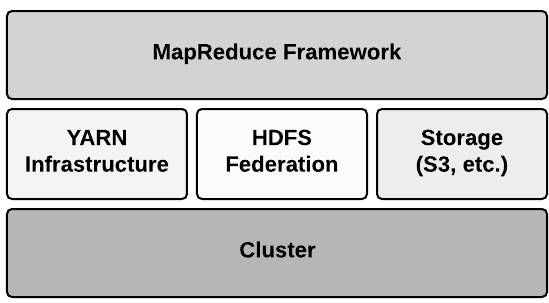
\includegraphics[width=\linewidth]{images/hadoop-architecture2.jpg}}
\caption{Hadoop Components \cite{www-hadooparch2}}
\label{fig:hadoop-components}
\end{figure}

Figure \ref{fig:hadoop-cluster} depicts a simple multi-node Hadoop cluster. The cluster contains master and slave nodes.  The master node contains a DataNode, a NameNode, a Job Tracker, and a Task Tracker. The slave node functions as both a Task Tracker and a Data Node \cite{www-hadooparch2}.

\begin{figure}[htbp]
\centering
\fbox{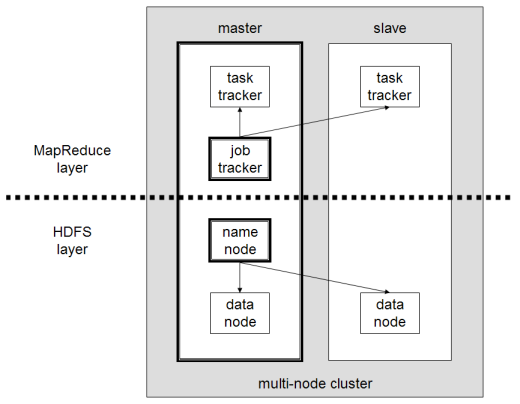
\includegraphics[width=\linewidth]{images/hadoop-architecture.png}}
\caption{Hadoop Cluster \cite{www-wikihadoop}}
\label{fig:hadoop-cluster}
\end{figure}


% https://en.wikipedia.org/wiki/Apache_Hadoop

\subsection{Apache Hama}

Apache Hama is a top level project in the Apache Software stack developed by Edward J Yoon.  Hama utilizes  Bulk Synchronous Parallel (BSP) to allow massive scientific computation \cite{www-wikihama}. 

Figure \ref{fig:hama-arch} details the architecture of Apache Hama.  Three key components are BSPMaster, ZooKeeper, and GroomServer. BSPMaster has several responsibilities including maintaining and scheduling jobs and communicating with the groom servers.  Groom Servers are processes that perform tasks assigned by BCPMaster.  Zookeeper efficiently manages synchronization of BSPPeers, instances started by groom servers \cite{www-wikihama}. 


\begin{figure}[htbp]
\centering
\fbox{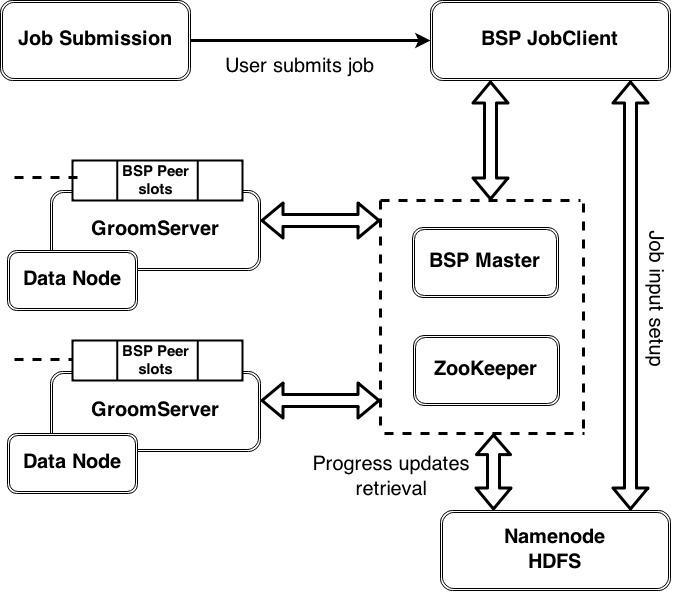
\includegraphics[width=\linewidth]{images/hama-architecture.jpg}}
\caption{Hama Architecture \cite{apachehama}}
\label{fig:hama-arch}
\end{figure}

% https://en.wikipedia.org/wiki/Apache_Hama


% fix this reference in sample.bib later

% https://www.researchgate.net/publication/307451491_Researching_Apache_Hama_A_Pure_BSP_Computing_Framework


\subsection{Apache Spark}

Apache Spark is open source software, originally developed at the University of California at Berkeley and later donated to the Apache Software Foundation. Spark is a cluster computing framework providing parallelism and fault tolerance \cite{www-wikispark}.

Figure \ref{fig:spark-arch} shows the various components of Apache Spark.  Spark Core is central to Spark's architecture and provides APIs, memory management, fault recovery, storage capabilities, and other features. On top of Spark core are several packages.  Spark SQL allows the use of SQL for working with structured data.  Spark Streaming provides real time streaming capabilities.  MLlib and GraphX allow the use of machine learning and graph algorithms \cite{www-techstory}.

% http://spark.apache.org/docs/1.3.0/cluster-overview.html

% https://en.wikipedia.org/wiki/Apache_Spark
\begin{figure}[htbp]
\centering
\fbox{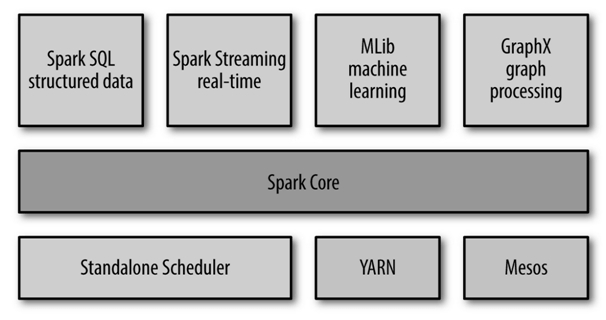
\includegraphics[width=\linewidth]{images/spark-architecture.jpg}}
\caption{Spark Architecture \cite{www-techstory}}
\label{fig:spark-arch}
\end{figure}

\subsection{Apache Flink}

Apache Flink is open source software developed by the Apache Software Foundation.  Flink features a "distributed streaming dataflow engine written in Java and Scala" \cite{www-wikiflink}.  Both batch and streaming processing programs can be executed on Flink.  Programs in Flink can be written in Java, Scala, Python, and SQL which are compiled and optimized and then executed on a Flink cluster.  Flink does not have an internal storage system and instead provides connectors to use with external sources like Amazon S3, Apache Kafka, HDFS, or Apache Cassandra \cite{www-wikiflink}.  Flink's full architechure is shown in Figure \ref{fig:flink-arch}.

% https://en.wikipedia.org/wiki/Apache_Flink

\begin{figure}[htbp]
\centering
\fbox{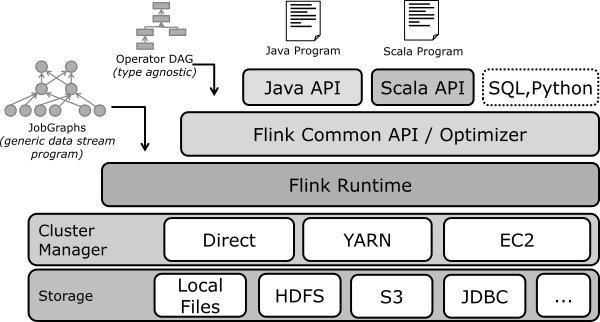
\includegraphics[width=\linewidth]{images/flink-architecture.jpg}}
\caption{Flink Architecture \cite{www-flinkarch}}
\label{fig:flink-arch}
\end{figure}

% https://ci.apache.org/projects/flink/flink-docs-release-0.7/internal_general_arch.html

\subsection{MRQL}

MRQL itself is made up of a core module, which includes data formats and structures used by MRQL.  Supporting modules, which sit on top of the core module, extend its functionalily \cite{mrqlthesis}.  MRQL uses a multi-step process to convert SQL statements to Jar files that are then deployed into the cluster.  SQL statements are first changed into MRQL algebraic form.  Next is a type interface step before the query is translated and normalized.  A plan is generated, simplified, normalized, and compiled into java btye code in the final jar file \cite{mrqlthesis}.

% https://uta-ir.tdl.org/uta-ir/bitstream/handle/10106/26371/PAUDEL-THESIS-2016.pdf?sequence=1

\section{MapReduce}

The MapReduce programing model was introduced by Google in 2004.  The MapReduce model involves a map and reduce function.  The map function processes key/value pairs to generate a new list of key/value pairs.  The reduce function merges these new values by key \cite{googlemapreduce}.  MapReduce Query Language is built upon the MapReduce model.  

% https://research.google.com/archive/mapreduce.html

\section{Language Features}

The MRQL language supports data types, functions, aggregation, and a SQL like syntax.

\subsection{Data Model}

MRQL is a typed language with several data types.  Basic types (bool, short, int, long, float, double, string), tuples, records, lists, bags, user-defined types, a data type T, and persistent collections are all supported by MRQL \cite{www-wikilanguage}. 

\subsection{Data Sources}

MRQL can access flat files (such as CSV) and XML and JSON documents \cite{www-wikilanguage}.

\subsection{Syntax}

MRQL supports a SQL like syntax.  MRQL includes group by and order by clauses, nested queries, and three types of repetition \cite{www-wikilanguage}.

\vspace{-\topsep}
\begin{verbatim}
select [ distinct ] e
from p1 in e1, ..., pn in en
[ where ec ]
[ group by p': e' [ having eh ] ]
[ order by e0 [ limit el ] ]
\end{verbatim}
%\vspace*{-\baselineskip}
\vspace{-\topsep}
\textbf{MRQL Select Query Syntax \cite{www-wikilanguage}}


\subsection{Functions and Aggregations}

In addition to predefined system functions, MRQL supports user defined functions and aggregations \cite{www-wikilanguage}.



\section{Licensing}

MRQL is open source software licensed under the Apache 2.0 software license \cite{www-mrqllicense}.

\section{Alternative Technologies}

There are several existing MapReduce Query Languages that are alternatives to MRQL.  Apache Hive (HiveQL), Apache Pig (Pig Latin), and JAQL, a JSON based query language originally developed by Google \cite{www-wikijaql}, are three examples.  Hive and Pig, popular Apache technologies, are explored in more detail.

\subsection{HiveQL - Apache Hive}

Apache Hive allows the use of the use of SQL (via HiveQL) to access and modify datasets in distributed storage that integrates with Hadoop.  Hive also provides a procedural language, HPL-SQL \cite{www-apachehive}.

Comparing MRQL to Hive, we find several differences. Hive stores metadata in a Relational Database Management System while MRQL does not utilize metadata.  MRQL allows the use of Group By on arbitrary queries.  Hive does not allow the use of Group By on subqueries.  MRQL runs on Hadoop, Hama, Spark, and Flink while Hive works on Hadoop, Tez, and Spark.  MRQL is compatible with text, sequence, XML, and JSON file formats.  Hive is compatible with test, sequence, ORC, and RCFile formats.  MRQL allows iteration; Hive does not.  MRQL allows streaming; Hive does not \cite{www-mrqpresent}.


%http://events.linuxfoundation.org/sites/events/files/slides/mrql-apachecon15.pdf

\subsection{Pig Latin - Apache Pig}

Apache Pig was developed at Yahoo in 2006.  Like MRQL and Hive, Pig abstracts programming from Java MapReduce to a simpler format.  Pig's programming language is called Pig Latin.  As opposed to declarative languages where the programmer specifies what will be done like SQL, Hive, and MRQL, Pig Latin is a procedural language where the programmer specifies how the task will be accomplished \cite{www-wikipig}.

% https://en.wikipedia.org/wiki/Pig_(programming_tool)

\subsection{Ecosystem}

MRQL is part of the vast Apache ecosystem often used when working with Big Data.  Other technologies in the Apache Big Data stack closely related to MRQL are Hadoop, Hama, Spark, Flink, and HDFS.

\section{Use Cases}

Due to MRQL's relatively recent development and current status in the Apache incubator, real world use cases are difficult to find.  Since MRQL can be utilized with Hadoop, Hama, Spark, and Flink, it can be utilized in a wide variety of situations.  MRQL can be used for complex data analysis including PageRank, matrix factorization, and k-means clustering \cite{www-apacheincubator}.

\section{Educational Material}

Several excellent resources exist for learning more about MRQL.  The Apache Wiki contains several research papers and presentations on MRQL by its creator Leonidas Fegaras and others \cite{www-wikiapache} which provide a theoretical bases for understanding MRQL.  Key resources are \emph{Apache MRQL (incubating): Advanced Query Processing for Complex, Large-Scale Data Analysis} by Leonidas Fegaras \cite{www-mrqpresent}, \emph{Supporting Bulk Synchronous Parallelism in Map-Reduce Queries} by Leonidas Fegaras \cite{wikibsp}, and \emph{An Optimization Framework for Map-Reduce Queries} by Leonidas Fegaras, Chengkai Li, and Upa Gupta \cite{wikiopt}.



The Apache Wiki also contains a \emph{Getting Started} page \cite{www-wikiastart} which describes steps such as downloading and installing MRQL, a detailed \emph{Language Description} \cite{www-wikilanguage}, and a listing of \emph{System Functions} \cite{www-wikifunctions}.  These are the best resources for hands on use of MRQL.

As MRQL is an open source technology, the source code it freely available.  It is stored in github \cite{www-gitmrql}.


\section{Conclusion}

MapReduce Query Language simplifies the popular MapReduce programing model frequently utilized with Big Data.  MRQL is powerful enough to express complex data analysis including PageRank, matrix factorization, and k-means clustering, yet due to its familiar SQL like syntax can be utilized by a wider variety of users without strong programming skills.

MRQL can be used with Apache Hadoop, Hama, Spark, and Flink. With Hadoop now a mainstream technology and Hama, Spark, and Flink important pieces of the Apache Big Data stack, potential applications of MRQL are wide ranging.

The declarative MRQL language is easy to use, yet powerful, featuring multiple data types, data sources, functions, aggregations, and a SQL like syntax, including order by, group by, nested queries, and repetition. 

While currently still an incubator project at Apache, MRQL shows promise as a rich, easy to use language with the flexibility of working with Hadoop, Hama, Spark, and Flink.  Due to these strengths, MRQL may emerge as a viable alternative to currently more popular high level MapReduce abstractions such as Hive and Pig.


% Bibliography

\bibliography{references}
 
\section*{Author Biography}
\begingroup
\setlength\intextsep{0pt}
\begin{minipage}[t][3.2cm][t]{1.0\columnwidth} % Adjust height [3.2cm] as required for separation of bio photos.
%  \begin{wrapfigure}{L}{0.25\columnwidth}
%   
\includegraphics[width=0.25\columnwidth]{images/john_smith.eps}
%  \end{wrapfigure}
  \noindent
  {\bfseries Mark McCombe} received his B.S. (Business Administration/Finance) and M.S. (Computer Information Systems) from Boston University.  He is currently studying Data Science at Indiana University Bloomington.
\end{minipage}
\endgroup

\newpage

\appendix

\section{Work Breakdown}

All work on this paper was completed solely by Mark McCombe.

\end{document}

